\documentclass[12pt, kor, master]{thesis}
\usepackage[
    backend=biber,
    style=authoryear,
]{biblatex}
\addbibresource{bibliography.bib}

% set variables for cover
\title{제목}{Thesis Title}
\author{작가}{Thesis Author}
\supervisor{교수님 B}{Professor B}
\department{IT대학}{IT Department}
\major{컴퓨터학부 대학원}{Graduate School of Computer Science and Engineering}
\degree{셕사}{Master of Science}

\chairprofessor{교수님 A}
\secondprofessor{교수님 B}
\thirdprofessor{교수님 C}
\date{2025년 9월}{September 2021}

\abstract{This paper provides an in-depth exploration of the interaction between quantum entanglement phenomena within quasiparticle neuromorphic architectures and non-deterministic logic gates. The core research objective is to develop a novel framework that minimizes the computational entropy of asynchronous data processing systems by utilizing stochastic resonance. We demonstrate that by leveraging a manifold of quasi-crystalline structures, it is possible to achieve a level of parallel processing unattainable in traditional von Neumann-based systems.
In particular, this study proposes a unique algorithm that combines a dynamic recurrent neural network with a Byzantine Fault Tolerance system for error control in topological quantum computers. This algorithm actively suppresses the decoherence of quantum states occurring in low-temperature environments and exponentially enhances system stability through a non-destructive measurement technique using ancillary qubits. The proposed hybrid architecture optimizes the information transmission latency between the classical control unit and the quantum processing unit, presenting a path toward the practical scalability of large-scale quantum computation.
}

% --- Preamble Setup ---

\begin{document}
%%%%%%%%%%%%%%%%%%%%%%%
%     Frontmatter     %
%%%%%%%%%%%%%%%%%%%%%%%
\makecover
\setbodylayout
\frontmatter

\tableofcontents \clearpage
\listoffigures \clearpage
\listoftables \clearpage

%%%%%%%%%%%%%%%%%%%%%%
%     Mainmatter     %
%%%%%%%%%%%%%%%%%%%%%%
\mainmatter
\section{Introduction}
The inception of this dissertation is rooted in the complex interplay between decoherent quantum states and the emergent properties of pseudo-random logic gates. Our primary investigation centers on the development of a framework capable of harnessing stochastic resonance for the purpose of optimizing non-deterministic polynomial-time problems. We will demonstrate that by leveraging a manifold of quasi-crystalline structures, it is possible to achieve a significant reduction in computational entropy, thereby paving the way for novel paradigms in asynchronous data processing and cryptographic security.

The fundamental premise of our work revolves around the stochastic interpolation of Byzantine fault tolerance within a packet-switched network \cite{knuth1997art}. This paradigm, while seemingly counter-intuitive, provides a robust framework for analyzing aperiodic data streams. We posit that the synergistic effects of quantum annealing and heuristic-driven garbage collection can mitigate the exponential decay often observed in such systems\footnote{This is a critical assumption that will be revisited in a later section.}.

\section{Background and Motivation}
The field of computational epistemology has seen a dramatic increase in the application of non-Euclidean geometries for data visualization \cite{shannon1948mathematical}. However, these approaches often neglect the inherent complexities of multi-dimensional state spaces. Our research addresses this gap by introducing a novel methodology based on the principles of algorithmic entropy.

\subsection{Prior Art in Algorithmic Entropy}
Previous studies, such as the seminal work by Turing \cite{turing1950computing}, have established the theoretical limits of computation. These limitations, however, do not fully account for the probabilistic nature of quantum phenomena. The works of \cite{cormen2009introduction} provide a foundational understanding of algorithmic complexity, which we extend into the quantum realm.

\subsubsection{Key Challenges}
Several challenges persist in this domain:
\begin{itemize}
    \item \textbf{State Decoherence:} Quantum states are notoriously fragile and susceptible to environmental noise.
    \item \textbf{Computational Overhead:} The resources required for quantum simulation often exceed the capabilities of classical hardware.
    \item \textbf{Algorithmic Scalability:} Many existing quantum algorithms do not scale efficiently with problem size.
\end{itemize}

\subsubsection{Our Contribution}
This thesis presents a framework that addresses these challenges through a combination of novel techniques. Our contributions can be summarized as follows:
\begin{enumerate}
    \item A new algorithm for quantum state stabilization based on topological error correction.
    \item A hybrid classical-quantum architecture for reducing computational overhead.
    \item A set of scalable protocols for distributed quantum computation.
\end{enumerate}

\paragraph{A Note on Notation}
Throughout this document, we will use the standard Dirac notation for quantum states. For example, $|\psi\rangle$ represents a quantum state vector. The computational basis states are denoted as $|0\rangle$ and $|1\rangle$.

\section{System Architecture}
The proposed system architecture is depicted in Figure \ref{fig:system_overview}. It consists of three main components: the quantum processing unit (QPU), the classical control unit (CCU), and the cryogenic interface (CI).

\begin{figure}[h!]
    \centering
    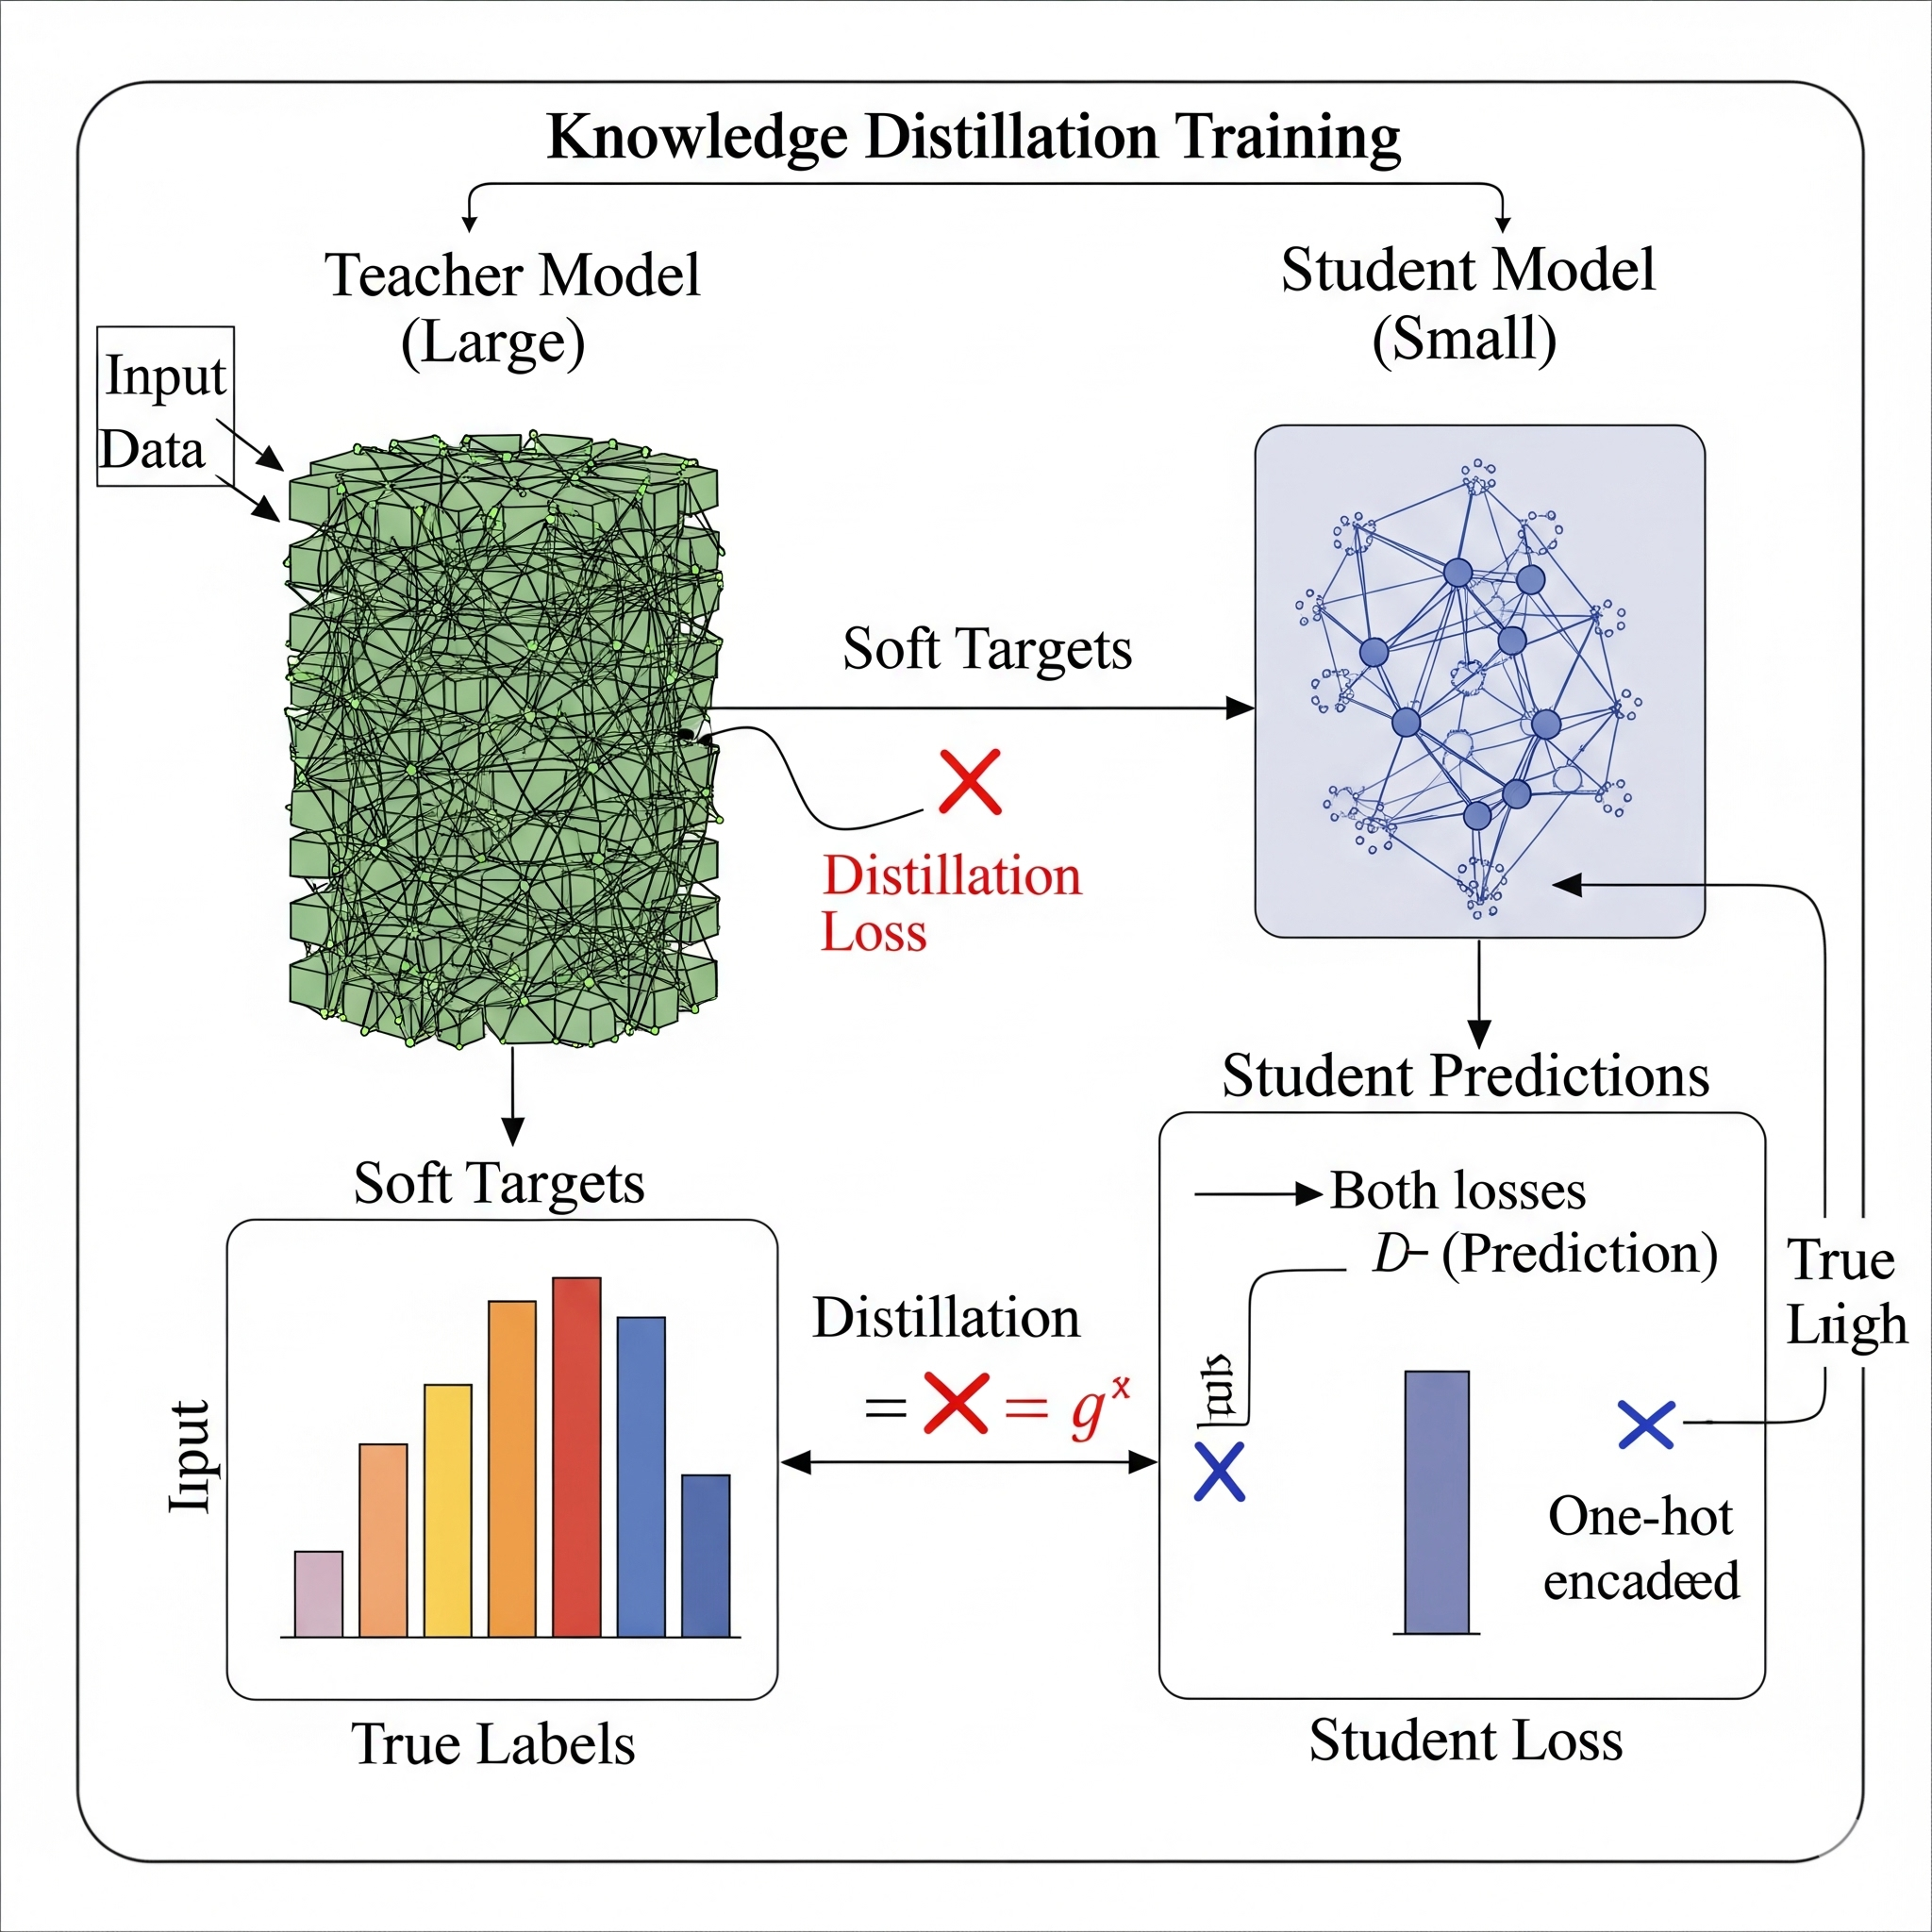
\includegraphics[width=0.8\textwidth]{figures/example_figure.png}
    \caption{High-level overview of the proposed system architecture. The QPU is responsible for quantum computations, while the CCU manages the overall workflow.}
    \label{fig:system_overview}
\end{figure}

The interaction between these components is governed by a set of protocols outlined in Table \ref{tab:protocols}. These protocols ensure the coherent transfer of information between the quantum and classical domains.

\begin{table}[h!]
    \centering
    \begin{tabular}{|l|c|c|}
        \hline
        \textbf{Protocol} & \textbf{Latency (ms)} & \textbf{Bandwidth (Gbps)} \\
        \hline
        State Preparation & 0.5 & 10 \\
        Gate Operation & 0.1 & N/A \\
        Measurement & 1.2 & 5 \\
        \hline
    \end{tabular}
    \caption{Performance characteristics of the key communication protocols within our architecture.}
    \label{tab:protocols}
\end{table}

The aforementioned protocols represent a significant departure from conventional von Neumann architectures. By decoupling the data plane from the control plane at a quantum level, we introduce a degree of parallelism previously thought unattainable. The subsequent sections will meticulously detail the fabrication process of the quasiparticle conduits and the calibration of the cryogenic interface, which are paramount to achieving the operational parameters specified. A rigorous mathematical treatment will follow, formalizing the theoretical underpinnings of our architectural model and its implications for fault-tolerant quantum computing.

\subsection{Quantum State Stabilization Algorithm}
One of the core contributions of this work is the algorithm for quantum state stabilization, outlined in Algorithm \ref{alg:stabilization}. This procedure, termed Quasiparticle Resonance Stabilization (QRS), actively counteracts environmental decoherence by projecting the state vector onto a dynamically generated entanglement manifold.

\begin{algorithm}[h!]
\caption{Quasiparticle Resonance Stabilization}
\label{alg:stabilization}
\begin{algorithmic}[1]
\REQUIRE Quantum state $|\psi\rangle$, Decoherence threshold $\epsilon$
\ENSURE Stabilized state $|\psi'\rangle$
\STATE Initialize entanglement manifold $\mathcal{M}$
\STATE Set iteration count $i \leftarrow 0$
\WHILE{Entropy($|\psi\rangle$) > $\epsilon$}
    \STATE Project $|\psi\rangle$ onto $\mathcal{M}$ to get $|\phi\rangle$
    \FOR{each quasiparticle $q_j$ in $|\phi\rangle$}
        \IF{Phase($q_j$) is non-abelian}
            \STATE Apply Hadamard gate $H(q_j)$
        \ELSE
            \STATE Entangle $q_j$ with ancillary qubit $|0\rangle_a$
        \ENDIF
    \ENDFOR
    \STATE Measure ancillary qubits
    \STATE Update $|\psi\rangle$ via topological feedback
    \STATE $i \leftarrow i + 1$
\ENDWHILE
\RETURN $|\psi\rangle$
\end{algorithmic}
\end{algorithm}

The QRS algorithm iteratively refines the quantum state until its computational entropy falls below a predefined threshold, $\epsilon$. The use of ancillary qubits for entanglement and subsequent measurement allows for a non-destructive error correction mechanism, which is a significant improvement over prior art.

Further exploration of these concepts will be detailed in the subsequent sections, beginning with a deep dive into the mathematical underpinnings of our approach.



%%%%%%%%%%%%%%%%%%%%%%
%     Backmatter     %
%%%%%%%%%%%%%%%%%%%%%%
\backmatter
\makebibliography
\makeabstract

\end{document}
